% University of Helsinki
% Department of Mathematics and Statistics
% Template for Bachelor's or Master's thesis
%
% This template is intended as a starting point for a thesis;
% feel free to customize it or use your own template.
% See the comments for hints and customization.
%
% Initial version: 29 August 2024 / Petri Laarne


% Add the 'twoside, openright' options when producing a proper printed version
\documentclass[a4paper, 11pt]{report}

\usepackage[hidelinks]{hyperref} % Always load this: clickable links and PDF reader navigation bar
\usepackage{lastpage} % Used to determine the total page count
\usepackage{calc} % For layout calculations involving TeX length units (template title page)
\usepackage{graphicx} % For embedding image files (JPEG, PNG, PDF)
\usepackage{subcaption} % For subfigures
\usepackage{tikz} % For drawing diagrams and other complex vector graphics

% If you use the LuaLaTeX or XeLaTeX compiler, comment out the following line.
% These compilers offer better support for Unicode, so you should use them if possible.
\usepackage[T1]{fontenc}

% Pass the language of the thesis as the LAST option in the list below.
% This changes the language used for dates and words like 'Chapter' or 'Bibliography'.
% You can remove the languages that do not appear in your work.
\usepackage[finnish,swedish,english]{babel}

\usepackage{csquotes} % This package is suggested by 'babel'

% Bibliography. Change the latter command if you modify the .bib file name.
\usepackage{biblatex}
\addbibresource{thesis-refs.bib}

\usepackage{mathtools} % Extended mathematics support (this package extends amsmath)
\usepackage{amssymb} % More mathematical symbols
\usepackage{amsfonts} % Blackboard bold mathematics font

% Theorem environments
\usepackage{amsthm}
\theoremstyle{plain}
\newtheorem{theorem}{Theorem}[section] % Theorems are numbered within chapter and section
\newtheorem{lemma}[theorem]{Lemma} % Lemmas etc. follow the same numbering as theorems
\theoremstyle{definition}
\newtheorem{definition}[theorem]{Definition}
\theoremstyle{remark}
\newtheorem{remark}[theorem]{Remark}

% Some examples of custom mathematical commands
\newcommand{\ZZ}{\mathbb Z} % Blackboard bold Z
\newcommand{\dx}{\mathop{}\!\mathrm d x} % Nice spacing (and upright d) for dx in integrals

% Finnish notation for evaluating integrals
% Instead of \int_a^b syntax you must use it as \sij{a}{b}
% (To enable the sub-/superscript syntax would require some more complicated TeX wizardry.)
\newcommand{\sij}[2]{\mathop{\bigg/}\nolimits_{\hspace{-0.65em}#1}^{\hspace{0.05em}#2}\hspace{-0.2em}}


\begin{document}

%
% TITLE PAGE
%
\begin{titlepage}

\noindent
\begin{minipage}[b]{\textwidth-45pt}
University of Helsinki\\
Faculty of Science\\
Insert DEGREE PROGRAMME name here
% Helsingin yliopisto\\
% Matemaattis-luonnontieteellinen tiedekunta\\
% Helsingfors universitet\\
% Matematisk-naturvetenskapliga fakulteten\\
\end{minipage}
\hfill
\includegraphics[width=45pt]{HYlogo.pdf}

\vspace{4pt}\hrule\vfill

\begin{center}
Bachelor's thesis / Master's thesis\\[8pt]
% Kandidaatintutkielma / Maisterintutkielma\\[8pt]
% Kandidatavhandlingen / Magisteravhandlingen\\[8pt]

{\huge\bfseries Title of the thesis}\\[8pt]

Firstname Lastname
\end{center}

\vfill\hrule\vspace{4pt}

\noindent
Supervisor:\hfill Month and year of submission\\
Firstname Lastname\\
Possible Other Supervisor
\end{titlepage}

%
% ABSTRACT
%
% This command starts a new page.
% In a print version ('twoside' option passed to \documentclass), the page is on the right side
\pagenumbering{gobble}
\cleardoublepage

\noindent\textbf{Title:} Repeat the title here\\ % Otsikko / Titel
\textbf{Author:} Your name here\\ % Tekijä / Författare
\textbf{Month and year:} Month and year of submission\\ % Aika / Datum
\textbf{Page count:} \pageref*{LastPage}~pp.\\[1em] % Sivumäärä: XX~s. / Sidoantal: XX~s.
% The page count is updated automatically, but it might require two compilations to be correct.
% If you customize the backmatter, this might become incorrect - check and correct manually if needed.

% If you include an abstract in a different language, wrap it in a foreignlanguage block
\begin{foreignlanguage}{english}
\noindent\textbf{Abstract:}\\ % Tiivistelmä / Referat
The abstract should be about one page long.
It also doubles as the maturity test.
Do not use mathematical notation in the abstract,
since it will also be displayed on the electronic thesis repository.

For the publication date, put in the month and year of submission of the finished thesis.
Also include 3~to 5~keywords that support searching for your thesis.
They are also shown one the repository page.

You can include the abstract in more than one language by copying and modifying
this code between comment blocks.
To get correct hyphenation for the language (and not with the rules of the main language),
put the text in a \verb|foreignlanguage| block as shown in the code
(just modify the language parameter to match the abstract).
\end{foreignlanguage}


\vfill

\noindent\textbf{Keywords:} Fill in some keywords, Separated by commas % Avainsanat / Nyckelord




%
% TABLE OF CONTENTS
%
\cleardoublepage
\tableofcontents


%
% MAIN TEXT STARTS HERE
%

% The \pagenumbering{arabic} command must be immediately after the first chapter title.
% Do not repeat it for other chapters.
\chapter{Introduction}
\pagenumbering{arabic}

\section{Compiling the document}

Depending on the language of your thesis, pass the correct option to the
\verb|\usepackage{babel}| command in the preamble.
This package changes all the built-in words (like \emph{Bibliography}) to the specified language.

If possible, you should use either the LuaLaTeX or XeLaTeX compiler to produce the PDF file.
You can change the compiler in the settings of your \LaTeX{} editor.
(In Overleaf, this setting is in the menu at the upper-left corner of screen.)

These compilers have better Unicode support than the old pdfLaTeX compiler,
and any future accessibility improvements will depend on these compilers.
If you use them, comment out the \verb|\usepackage{fontenc}| line
from the beginning of the document.


The bibliography is produced by a program called Biber.
Overleaf handles this automatically.
You can edit the \verb|.bib| source file for bibliography entries either manually%
\footnote{See Section~2 of the biblatex documentation at \url{https://ctan.org/pkg/biblatex}
for more information on the syntax.
The documentation also explains customization of the bibliography and citation styles.}
or export the file from a reference management program like Zotero.



\section{Figures and tables}

\LaTeX{} automatically ``floats'' figures and tables into a suitable position,
usually at the top of current or next page.
It is usually best to let the algorithm do its thing;
any manual tweaks are likely to break if the layout changes even by a tiny bit.

To create a figure, you can use the \verb|figure| environment.
You can create a cross-reference point (like Figure~\ref{fig:university logo})
by adding a label after the caption.
Note that the cross-reference above is clickable
-- this feature is provided by the `hyperref' package.

\begin{figure}
\centering

\includegraphics[width=0.4\textwidth]{HYlogo.pdf}
\caption{The emblem of University of Helsinki.
As it is a trademark of the university, its use is governed by some restrictions.}
\label{fig:university logo}
\end{figure}

To create subfigures as in Figure~\ref{fig:subfigures},
you can use the `subcaption' package.
It is possible to create subfigure references like Figure~\ref{sub}
by placing the label inside the subcaption definition.
(You can also create automatic, clickable references to the subfigure letter, like (\subref{sub})).

\begin{figure}
\centering

\subcaptionbox{The university logo.\label{sub}}{
\includegraphics[width=0.3\textwidth]{HYlogo.pdf}}
\subcaptionbox{Made a bit bigger.}{
\includegraphics[width=0.4\textwidth]{HYlogo.pdf}}
\subcaptionbox{And a bit smaller.}{
\includegraphics[width=0.2\textwidth]{HYlogo.pdf}}
\subcaptionbox{This goes on a new row.}{
\includegraphics[width=0.2\textwidth]{HYlogo.pdf}}

\caption{The subfigures are automatically placed in a grid.
Manual break points can be created with empty lines.}
\label{fig:subfigures}
\end{figure}

If you need to place a picture inline with text,
you can also do so, but then the picture is not numbered (and it might cause ugly page breaking).
Here the feature is illustrated with a simple diagram using the 'tikz' package.
TikZ is an extremely powerful package for making diagrams.
You can find a lot of examples online.

\begin{center}
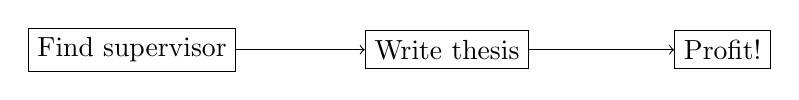
\begin{tikzpicture}

\node[draw] (A) at (0,0) {Find supervisor};
\node[draw] (B) at (4,0) {Write thesis};
\node[draw] (C) at (7.5,0) {Profit!};

\draw[->] (A.east) -- (B.west);
\draw[->] (B.east) -- (C.west);

\end{tikzpicture}
\end{center}


Like figures, there are also floating environments for tables.
Tables are numbered in their own sequence (like Table~\ref{tbl:theses}) by default.
Table contents are set with a \verb|tabular| environment.

\begin{table}
\centering
\begin{tabular}{r|lcc}
Dissertation & Shorthand & Typical length & Credits\\
\hline
Bachelor's & BSc & 10--20 pages & 6~cr\\
Master's & MSc & 30--50 pages & 30~cr\\
Doctoral & PhD & 3 articles + intro & N/A
\end{tabular}
\caption{Various academic dissertations in mathematics.}
\label{tbl:theses}
\end{table}

For better automatic handling of cross-references (although only in English-language text),
you can look at the `cleveref' package\footnote{\url{https://ctan.org/pkg/cleveref}}.



\section{Mathematics}

This example equation illustrates some custom commands defined in the document preamble:
\begin{equation}\label{eq:example}
\int_0^{2\pi} \sin(x + k\pi) \dx = -\sij{0}{2\pi} \cos(x) = 0,
\quad k \in \ZZ.
\end{equation}
In particular, the \verb|\dx| command ensures good spacing (and upright `d') of $\dx$ within the integral.
(The middle notation is only used in Finland.)

To create an unnumbered display equation like
\[
a^2 + b^2 = c^2,
\]
use the \verb|\[ \]| syntax or \verb|equation*| environment.
The old \TeX{} syntax \verb|$$ $$| is not fully compatible
with modern \LaTeX{} enhancements.

Remember that equations are part of text,
so you should put punctuation (like \verb|.| and \verb|,|)
inside equation environments if necessary.
For inline mathematics like $a^2 + b^2$, keep the punctuation outside the dollar signs.
Do not put empty lines around equation environments unless
there is supposed to be a paragraph break.

\bigskip

To find a particular mathematical symbol,
the Detexify tool\footnote{\url{https://detexify.kirelabs.org/}} is super useful.
It lets you draw a symbol, and suggests similar symbols from base \LaTeX{} and common packages.
Common symbols are also listed in the mathematics section of
\LaTeX{} Wikibook\footnote{\url{https://en.wikibooks.org/wiki/LaTeX/Mathematics}}.

Equations are numbered within chapter by default.
They too can be cross-referenced, like \eqref{eq:example}.
There are several other equation environments, like the one that aligns lines
(each line is numbered except for one, and one of them has a special name):
\begin{align}
\left( \sum_{k=0}^2 a^{2-k} b^k \right) (a-b)
&= (a^2 + ab + b^2) (a - b) \label{eq:second}\\
&= a^3 - a^2 b + a^2 b - ab^2 + b^2 a - b^3 \label{eq:third}\\
&= a^3 - (a^2 b - a^2 b) - (ab^2 - a b^2) - b^3 \notag\\
&= a^3 - b^3. \tag{AB}\label{eq:AB}
\end{align}
The lines can be referred to as \eqref{eq:second}, \eqref{eq:third}, and \eqref{eq:AB}.


\section{Theorems, definitions, and proofs}

The preamble defines some theorem-like environments with different styles.
You can create more such environments and change their names by modifying the code there.

These environments are numbered within chapter and section.
If you'd prefer to not reset the numbering in each section
(that is, Definition~1.1 instead of Definition~1.4.1),
you can change the indicated line in the preamble.

\begin{definition}
A triple $(a, b, c)$ of positive integers is called \emph{Pythagorean} if $a^2 + b^2 = c^2$.
\end{definition}

It is possible to give a name to such a block.

\begin{lemma}[A very silly lemma]
There exists at least one Pythagorean triple.
\end{lemma}
\begin{proof}
Pick $(a, b, c) = (3, 4, 5)$.
\end{proof}

If you want the block name to refer to a result in a published work,
you need to wrap the citation command in \verb|{{}}|.
This is due to some unfortunate \TeX nical details.

\begin{theorem}[{{\cite[Theorem~0.5]{wiles}}}]
There does not exist a triple $(a, b, c)$ of positive integers such that $a^3 + b^3 = c^3$.
\end{theorem}
\begin{proof}
Left as an exercise to the reader.
\end{proof}

\begin{remark}
The last proof was a joke.
\end{remark}



\section{Citing literature}

Use the \verb|\cite| command to cite entries from the \verb|.bib| file,
like \cite{analyysia}.
You can also use an optional argument to cite a specific part, like \cite[p.~20]{analyysia}.

Only cited entries are included in the final bibliography.
To force the inclusion of all entries (for testing purposes!),
you can add \verb|\nocite{*}| somewhere in the code.
\nocite{*}

Refer to the biblatex documentation \cite{biblatex}
for changing the appearance of citations and the bibliography.
The \verb|.bib| file attached to this template shows the basic elements
of various entry types.

Reference management programs like Zotero support exporting \verb|.bib| files.
You can also download citations from \mbox{zbMATH}, Google~Scholar, and most journals
directly in \verb|.bib| format.

One more note: Some bibliography styles may change the capitalization of words.
Use \verb|{}| to protect specific words from this behaviour,
like \verb|{Fermat's}| in the entry for \cite{wiles}.




%
% BIBLIOGRAPHY
%
% The [heading=bibintoc] option adds the bibliography to table of contents
\printbibliography[heading=bibintoc]




%
% APPENDICES (if necessary)
%
\appendix

\chapter{Some more information}

If you need to have appendices in your thesis,
you can write them as usual chapters after the \verb|\appendix| command.
Appendices are numbered alphabetically.

\end{document}
